\input{head.inc}
\usepackage{tikz-3dplot}
\usetikzlibrary{shapes.geometric}
\newcommand{\Tube}[6][]%
% [further options], width, iterations, inner color, outer color, path definition
{   \colorlet{InColor}{#4}
    \colorlet{OutColor}{#5}
    \foreach \I in {1,...,#3}
    {   \pgfmathsetlengthmacro{\h}{(\I-1)/#3*#2}
        \pgfmathsetlengthmacro{\r}{sqrt(pow(#2,2)-pow(\h,2))}
        \pgfmathsetmacro{\c}{(\I-0.5)/#3*100}
        \draw[InColor!\c!OutColor, line width=\r, #1] #6;
    }
}

% Präambelbefehle für die Präsentation
\title[TET: Antennen I - Hertzscher Dipol und Linearantennen]{TET: Antennen I - Hertzscher Dipol und Linearantennen}

\begin{document}
% 
% Frontmatter 
% 
%%%%%%%%%%%%%%%%%%%%%%%%%%%%%%%%%%%%%%%%%%%%%%%%%%%%%%%%%%%%%%%%%%%%%%%%%%%%%%%%%%%%%%%%%%%%%%%%%%%%%%%%%%%%%%%%%%%%%%%%%%%%% 

%% inserts the title page and the table of contents
\maketitle

% 
% Content 
% 
%%%%%%%%%%%%%%%%%%%%%%%%%%%%%%%%%%%%%%%%%%%%%%%%%%%%%%%%%%%%%%%%%%%%%%%%%%%%%%%%%%%%%%%%%%%%%%%%%%%%%%%%%%%%%%%%%%%%%%%%%%%%% 
\section{TET: Antennen I - Hertzscher Dipol und Linearantennen}

\begin{frame}
  \frametitle{Ausgangspunkt}

  \begin{columns}
    \begin{column}{.35\textwidth}
  % set the plot display orientation
%synatax: \tdplotsetdisplay{\theta_d}{\phi_d}
\tdplotsetmaincoords{60}{110}

%define polar coordinates for some vector
%TODO: look into using 3d spherical coordinate system
\pgfmathsetmacro{\rvec}{.5}
\pgfmathsetmacro{\thetavec}{30}
\pgfmathsetmacro{\phivec}{60}

%start tikz picture, and use the tdplot_main_coords style to implement the display 
%coordinate transformation provided by 3dplot
\begin{tikzpicture}[scale=5,tdplot_main_coords]

%set up some coordinates 
%-----------------------
\coordinate (O) at (0,0,0);

%determine a coordinate (P) using (r,\theta,\phi) coordinates.  This command
%also determines (Pxy), (Pxz), and (Pyz): the xy-, xz-, and yz-projections
%of the point (P).
%syntax: \tdplotsetcoord{Coordinate name without parentheses}{r}{\theta}{\phi}
\tdplotsetcoord{P}{\rvec}{\thetavec}{\phivec}

%draw figure contents
%--------------------

%draw the main coordinate system axes
\draw[thick,->] (0,0,0) -- (.5,0,0) node[anchor=north east]{$x$};
\draw[thick,->] (0,0,0) -- (0,.5,0) node[anchor=north west]{$y$};
\draw[thick,->] (0,0,0) -- (0,0,.5) node[anchor=south]{$z$};

%draw a vector from origin to point (P) 
\draw[-stealth,color=red,thick] (O) -- (P) node[midway, below]{$\ortsvektor[v]$};
\draw[-stealth,color=green,thick] (P) -- +(0,0,0.2) node[above]{$\magvekpot[uv]=\magvekpot[u]_z\einheitsvek{z}$};

%draw projection on xy plane, and a connecting line
\draw[dashed, color=red] (O) -- (Pxy);
\draw[dashed, color=red] (P) -- (Pxy);

%draw the angle \phi, and label it
%syntax: \tdplotdrawarc[coordinate frame, draw options]{center point}{r}{angle}{label options}{label}
\tdplotdrawarc{(O)}{0.2}{0}{\phivec}{anchor=north}{$\varphi$}


%set the rotated coordinate system so the x'-y' plane lies within the
%"theta plane" of the main coordinate system
%syntax: \tdplotsetthetaplanecoords{\phi}
\tdplotsetthetaplanecoords{\phivec}

%draw theta arc and label, using rotated coordinate system
\tdplotdrawarc[tdplot_rotated_coords]{(0,0,0)}{0.3}{0}{\thetavec}{anchor=south west}{$\vartheta$}

%draw some dashed arcs, demonstrating direct arc drawing
%\draw[dashed,tdplot_rotated_coords] (\rvec,0,0) arc (0:90:\rvec);
%\draw[dashed] (\rvec,0,0) arc (0:90:\rvec);

%set the rotated coordinate definition within display using a translation
%coordinate and Euler angles in the "z(\alpha)y(\beta)z(\gamma)" euler rotation convention
%syntax: \tdplotsetrotatedcoords{\alpha}{\beta}{\gamma}
\tdplotsetrotatedcoords{\phivec}{\thetavec}{0}

%translate the rotated coordinate system
%syntax: \tdplotsetrotatedcoordsorigin{point}
\tdplotsetrotatedcoordsorigin{(P)}

%use the tdplot_rotated_coords style to work in the rotated, translated coordinate frame
\draw[thin,tdplot_rotated_coords,->] (0,0,0) -- (.1,0,0) node[anchor=north west]{$\vu{\vartheta}$};
\draw[thin,tdplot_rotated_coords,->] (0,0,0) -- (0,.1,0) node[anchor=west]{$\vu{\varphi}$};
\draw[thin,tdplot_rotated_coords,->] (0,0,0) -- (0,0,.1) node[anchor=south]{$\vu{r}$};

\node (a) [cylinder, shape border rotate=90, draw, minimum height=5mm, minimum width=2mm,yshift=-1mm] {};
\draw [<->] ([xshift=-2pt]a.before bottom) -- ([xshift=-2pt]a.after top) node [midway, left] {$\ell$};

\end{tikzpicture}
\end{column}
\begin{column}{.65\textwidth}
  \begin{itemize}[<+->]
  \item Der \alert{Hertzsche Dipol} ist eine wichtige Idealisierung einer lokalen Quelle von elektromagnetischen Wellen.
    \item Hertzsche Dipole werden auch in der Modellierung von Antennen und als Bezugsgröße für Antennencharakteristiken genutzt.
    \item Realisiert wird der Hertzsche Dipol durch einen sehr kurzen geraden Leiter, auf dem ein Wechselstrom (in der Regel harmonisch) eingeprägt ist.
      \end{itemize}
\end{column}
\end{columns}
  \begin{itemize}[<+->]
    \item Für harmonische Zeitabhängigkeit gilt für das Vektorpotential in Lorenzeichung
      \begin{equation*}
        \magvekpot[uv](\ortsvektor[v]) = \frac{\mu}{4\pi} \iiint_V \frac{\euler^{-\komplex\wellenzahl|\ortsvektor[v]-\ortsvektor[vs]|}}{|\ortsvektor[v]-\ortsvektor[vs]|} \elstromdichte[uv](\ortsvektor[vs]) \upd^3 \ortsvektor[s]
        \end{equation*}
    \item Mit einem \alert{dünnen Leiter} in \(z\)-Richtung gilt \(\elstromdichte[uv](\ortsvektor[vs]) \upd^3 \ortsvektor[s] = \underline{I}(\ortsvektor[vs])\einheitsvek{z}\upd z^\prime \) und es folgt
      \begin{equation*}
        \magvekpot[uv](\ortsvektor[v]) = \frac{\mu}{4\pi} \int_{-\nicefrac{\ell}{2}}^{\nicefrac{\ell}{2}} \frac{\euler^{-\komplex\wellenzahl |\ortsvektor[v]-\ortsvektor[vs]|}}{|\ortsvektor[v]-\ortsvektor[vs]|} \underline{I}(\ortsvektor[vs])\einheitsvek{z}\upd z^\prime
        \end{equation*}
\end{itemize}
\end{frame}


\begin{frame}
  \frametitle{Hertzscher Dipol - Vektorpotential}
      \begin{equation*}
        \magvekpot[uv](\ortsvektor[v]) = \frac{\mu}{4\pi} \int_{-\nicefrac{\ell}{2}}^{\nicefrac{\ell}{2}} \frac{\euler^{-\komplex\wellenzahl |\ortsvektor[v]-\ortsvektor[vs]|}}{|\ortsvektor[v]-\ortsvektor[vs]|} \underline{I}(\ortsvektor[vs])\einheitsvek{z}\upd z^\prime
        \end{equation*}
  \begin{itemize}[<+->]
  \item Von einem \alert{Hertzschem Dipol} spricht man, wenn
    \begin{enumerate}
    \item Die Länge \(\ell\) des Leiters \alert{wesentlich kleiner als die Wellenlänge} \(\lambda\) ist: \(\ell \ll \lambda\)
    \item Der Leiter ist \alert{linienförmig}.
      \item Die Stromverteilung auf dem Leiter ist \alert{konstant}: \(\underline{I}(\ortsvektor[vs]) = \underline{I} \)
      \end{enumerate}
    \item Für einen \alert{Dipol im Ursprung}: \(\ortsvektor[vs] \simeq \vec{0} \to |\ortsvektor[v]-\ortsvektor[vs]| \simeq |\ortsvektor[v]|=\ortsvektor\)
      \begin{equation*}
        \boxed{\magvekpot[uv](\ortsvektor[v]) = \frac{\mu}{4\pi} \frac{\euler^{-\komplex\wellenzahl\ortsvektor}}{\ortsvektor} \underline{I}\einheitsvek{z}\int_{-\nicefrac{\ell}{2}}^{\nicefrac{\ell}{2}} \upd z^\prime = \frac{\mu}{4\pi} \underline{I} \ell  \frac{\euler^{-\komplex\wellenzahl\ortsvektor}}{\ortsvektor} \einheitsvek{z}} = \magvekpot[u]_z \einheitsvek{z} 
        \end{equation*}
      \item Vektorpotential in Kugelkoordinaten \((r,\vartheta,\varphi)\):
        \begin{align*}
          \magvekpot[u]_r &=  \magvekpot[u]_z \cos\vartheta & \magvekpot[u]_\vartheta &=  -\magvekpot[u]_z \sin\vartheta & \Aboxed{\magvekpot[u]_\varphi &=0}\\
          \Aboxed{\magvekpot[u]_r &=  \frac{\mu}{4\pi} \underline{I} \ell  \frac{\euler^{-\komplex\wellenzahl\ortsvektor}}{\ortsvektor} \cos\vartheta} & \Aboxed{\magvekpot[u]_\vartheta &=  - \frac{\mu}{4\pi} \underline{I} \ell  \frac{\euler^{-\komplex\wellenzahl\ortsvektor}}{\ortsvektor} \sin\vartheta} & &  
          \end{align*}
  \end{itemize}
\end{frame}

\begin{frame}
  \frametitle{Magnetfeld}
  \begin{itemize}[<+->]
\item Aus dem Vektorpotential
        \begin{align*}
          \magvekpot[u]_r &=  \frac{\mu}{4\pi} \underline{I} \ell  \frac{\euler^{-\komplex\wellenzahl\ortsvektor}}{\ortsvektor} \cos\vartheta & \magvekpot[u]_\vartheta &=  -\frac{\mu}{4\pi} \underline{I} \ell  \frac{\euler^{-\komplex\wellenzahl\ortsvektor}}{\ortsvektor} \sin\vartheta & \magvekpot[u]_\varphi &=0  
          \end{align*}
  \item berechnet sich unmittelbar das Magnetfeld:
    \begin{align*}
      \magfeld[uv] &= \magfeld[u]_\varphi \einheitsvek{\varphi} = \frac{1}{\mu} \rotation\magvekpot[uv] = \frac{1}{\mu} \frac{1}{r} \left[ \frac{\d \left(r \magvekpot[u]_\vartheta  \right)}{\d r} - \frac{\d \magvekpot[u]_r}{\d \vartheta} \right] \einheitsvek{\varphi} \text{ nur \(\varphi\)-Komponente} \\
      &= \frac{1}{4\pi} \underline{I} \ell  \frac{\euler^{-\komplex\wellenzahl\ortsvektor}}{\ortsvektor}\sin\vartheta \left[\frac{1}{\ortsvektor} + \komplex\wellenzahl\right]\; \einheitsvek{\varphi}\\  
                                                                                                       &= \frac{1}{4\pi} \underline{I} \ell  \frac{\euler^{-\komplex\wellenzahl\ortsvektor}}{\ortsvektor^2} \sin\vartheta \left[1+\komplex \wellenzahl \ortsvektor \right]\; \einheitsvek{\varphi} \quad \wellenzahl = \nicefrac{\omega}{\geschw_p}\\
      &= \frac{1}{4\pi} \frac{\omega^2}{\geschw_p^2}\underline{I} \ell  \frac{\euler^{-\komplex\wellenzahl\ortsvektor}}{(\wellenzahl\ortsvektor)^2} \sin\vartheta \left[1+\komplex \wellenzahl \ortsvektor \right]\; \einheitsvek{\varphi} = \frac{1}{4\pi} \frac{\omega^2}{\geschw_p^2}\underline{I} \ell  \euler^{-\komplex\wellenzahl\ortsvektor} \sin\vartheta \left[\frac{1}{(\wellenzahl\ortsvektor)^2}+ \frac{\komplex}{\wellenzahl \ortsvektor} \right]\; \einheitsvek{\varphi}
    \end{align*}
    \item \(\wellenzahl \ortsvektor = 2\pi\frac{\ortsvektor}{\lambda}\): Wellenlänge als \enquote{natürliche} Längeneinheit
  \end{itemize}
\end{frame}


\begin{frame}
  \frametitle{Elektrisches Feld}
  \begin{itemize}[<+->]
  \item Das Elektrische Feld könnte prinzipiell auch direkt aus dem Vektorpotential berechnet werden:
    \begin{align*}
      \text{LE: } \divergenz\magvekpot[uv] + \komplex \omega \varepsilon\mu \elpotential[u]  = 0 &\Rightarrow \elpotential[u] = -\frac{1}{\komplex \omega \varepsilon\mu} \divergenz\magvekpot[uv]\\
      \efeld[uv] = -\gradient \elpotential[u] - \komplex \omega \magvekpot[uv] &\Rightarrow \efeld[uv]  = \frac{1}{\komplex \omega \varepsilon\mu} \gradient \divergenz\magvekpot[uv]- \komplex \omega \magvekpot[uv]    
    \end{align*}
  \item Einfacher direkt über Maxwell-Gleichung
    \begin{equation*}
      \rotation \magfeld[uv] = \elstromdichte[uv] + \komplex\omega\varepsilon\efeld[uv] \Rightarrow \efeld[uv] = \frac{1}{\komplex\omega\varepsilon} \rotation \magfeld[uv] \quad \elstromdichte[uv] = \vec{0} \text{ im Lösungsgebiet} 
    \end{equation*}
  \item Es ergibt sich
    \begin{align*}
      \efeld[uv] = &\left\{\frac{1}{2\pi} Z \frac{\omega^2}{\geschw_p^2}\underline{I} \ell  \euler^{-\komplex\wellenzahl\ortsvektor} \cos\vartheta\left[\frac{1}{(\wellenzahl\ortsvektor)^2} - \frac{\komplex}{(\wellenzahl\ortsvektor)^3}\right]\right\} \einheitsvek{r} + \\
      &\left\{ \frac{1}{4\pi} Z \frac{\omega^2}{\geschw_p^2}\underline{I} \ell  \euler^{-\komplex\wellenzahl\ortsvektor} \sin\vartheta\left[\frac{\komplex}{\wellenzahl\ortsvektor}  + \frac{1}{(\wellenzahl\ortsvektor)^2} - \frac{\komplex}{(\wellenzahl\ortsvektor)^3} \right] \right\} \einheitsvek{\vartheta}
      \end{align*}
  \end{itemize}
\end{frame}

\begin{frame}
  \frametitle{Fernfeld}
  \begin{itemize}[<+->]
  \item Die allgemeine Feldlösung lautet:
    \begin{align*}
            \magfeld[uv] = &\left\{\frac{1}{4\pi} \frac{\omega^2}{\geschw_p^2}\underline{I} \ell  \euler^{-\komplex\wellenzahl\ortsvektor} \sin\vartheta \left[\frac{1}{(\wellenzahl\ortsvektor)^2}+ \frac{\komplex}{\wellenzahl \ortsvektor} \right]\right\}\; \einheitsvek{\varphi}\\
      \efeld[uv] = &\left\{\frac{1}{2\pi} Z \frac{\omega^2}{\geschw_p^2}\underline{I} \ell  \euler^{-\komplex\wellenzahl\ortsvektor} \cos\vartheta\left[\frac{1}{(\wellenzahl\ortsvektor)^2} - \frac{\komplex}{(\wellenzahl\ortsvektor)^3}\right]\right\}\; \einheitsvek{r} + \\
      &\left\{ \frac{1}{4\pi} Z \frac{\omega^2}{\geschw_p^2}\underline{I} \ell  \euler^{-\komplex\wellenzahl\ortsvektor} \sin\vartheta\left[\frac{\komplex}{\wellenzahl\ortsvektor}  + \frac{1}{(\wellenzahl\ortsvektor)^2} - \frac{\komplex}{(\wellenzahl\ortsvektor)^3} \right] \right\}\; \einheitsvek{\vartheta}
    \end{align*}
  \item Für \(\wellenzahl \ortsvektor \gg 1 \to\) nur führenden Term nehmen \(\to\) \alert{Fernfeld}
    \begin{align*}
            \Aboxed{\magfeld[uv]= \magfeld[u]_\varphi \; \einheitsvek{\varphi} = &\frac{\komplex}{4\pi} \frac{\omega^2}{\geschw_p^2}\underline{I} \ell  \frac{\euler^{-\komplex\wellenzahl\ortsvektor}}{\wellenzahl\ortsvektor} \sin\vartheta \; \einheitsvek{\varphi}}\\
      \Aboxed{\efeld[uv] = \efeld[u]_\vartheta \; \einheitsvek{\vartheta} = &Z \frac{\komplex}{4\pi} \frac{\omega^2}{\geschw_p^2}\underline{I} \ell  \frac{\euler^{-\komplex\wellenzahl\ortsvektor}}{\wellenzahl\ortsvektor} \sin\vartheta\; \einheitsvek{\vartheta}} = Z\; \magfeld[u]_\varphi \; \einheitsvek{\vartheta}
    \end{align*}
    \item Hierbei ist \(Z=\frac{|\efeld[uv]|}{|\magfeld[uv]|} = \sqrt{\frac{\mu}{\varepsilon}} = \frac{\wellenzahl}{\omega\varepsilon}\) der \alert{Feldwellenwiderstand}
    \end{itemize}
    \ 
\end{frame}


\begin{frame}
  \frametitle{Visualisierung}
  \begin{itemize}[<+->]
  \item R. Girwidz, Didaktik der Physik, LMU München \url{https://www.didaktikonline.physik.uni-muenchen.de/programme/dipolstr/Dipolstr_leifi.html}
  \centerline{\includegraphics[width=.75\textwidth]{Dipol-LMU}}
    \end{itemize}
  \end{frame}

\begin{frame}
  \frametitle{Mittlere Energieflussdichte}
  \begin{itemize}[<+->]
  \item Im Fernfeld berecht sich die \alert{mittlere Energieflussdichte} zu
    \begin{align*}
      \poyvec[uv] &= \frac{1}{2} \efeld[uv] \times \magfeld[uv]^\star = \frac{1}{2} \left( Z \frac{\komplex}{4\pi} \frac{\omega^2}{\geschw_p^2}\underline{I} \ell  \frac{\euler^{-\komplex\wellenzahl\ortsvektor}}{\wellenzahl\ortsvektor} \sin\vartheta\; \einheitsvek{\vartheta} \right) \times \left(\frac{\komplex}{4\pi} \frac{\omega^2}{\geschw_p^2}\underline{I} \ell  \frac{\euler^{-\komplex\wellenzahl\ortsvektor}}{\wellenzahl\ortsvektor} \sin\vartheta \; \einheitsvek{\varphi} \right)^\star\\
                  &= \frac{1}{2} Z \left( \frac{1}{4\pi} \frac{\omega^2}{\geschw_p^2}\frac{|\underline{I}| \ell}{\wellenzahl\ortsvektor} \right)^2 \left(\sin\vartheta\right)^2 \; \einheitsvek{r} \in \mathbb{R} \\
                    & = \poyvec_r(r,\vartheta) \; \einheitsvek{r} = \langle \poyvec[v] \rangle 
    \end{align*}
  \item Verlauf -- \enquote{Donut}
    \begin{columns}
      \begin{column}{.5\textwidth}
\hspace*{2cm}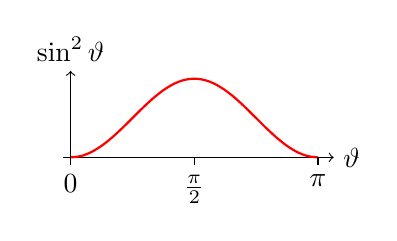
\begin{tikzpicture}
  \draw[->] (-.1, 0) -- (pi+0.2, 0) node[right] {$\vartheta$};
  \draw[->] (0, -0.1) -- (0, 1.1) node[above] {$\sin^2\vartheta$};
  \draw[domain=0:pi, smooth, variable=\x, red, thick] plot ({\x}, {(sin(\x*180/pi))^2});
  \draw[thin] (0,0) -- (0,-0.1) node[below]{$0$}; 
  \draw[thin] (pi/2,0) -- (pi/2,-0.1) node[below]{$\frac{\pi}{2}$}; 
  \draw[thin] (pi,0) -- (pi,-0.1) node[below]{$\pi$}; 
\end{tikzpicture}
\end{column}
      \begin{column}{.5\textwidth}
 \hspace*{1cm}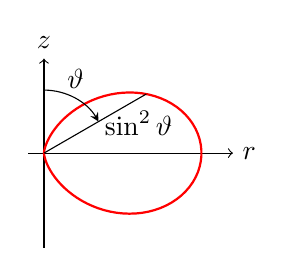
\begin{tikzpicture}[scale=2]
   \draw[->] (-.1, 0) -- (1.2, 0) node[right] {$r$};
   \draw[->] (0, -0.6) -- (0, 0.6) node[above] {$z$};
   % \draw[thick,red] (0,0) \foreach \th in {1, ... ,180} { -- ({90-\th}:{(sin(\th))^2}) };
   \draw[thick,red,variable=\th,domain=0:180,samples=90]
   plot ( {(sin(\th))^3} , {cos(\th)*(sin(\th))^2} );
   \draw [thin] (0,0) -- (30:{(sin(60))^2}) node[midway, right]{$\sin^2\vartheta$};
   \draw [thin,-stealth] (0,0.4) arc (90:30:0.4) node[midway,above]{$\vartheta$};
 \end{tikzpicture}
 \end{column}
\end{columns}
\end{itemize}
  \end{frame}

\begin{frame}
  \frametitle{Strahlungsdiagramm}
  \begin{itemize}[<+->]
  \item Das \alert{Strahlungsdiagramm} ist die normierte Darstellung der mittleren Energieflussdichte (analog z.B. auch für Feldstärken definierbar), also von
    \begin{equation*}
      \frac{\poyvec_r(r,\vartheta, \varphi)}{\max(\poyvec_r(r,\vartheta, \varphi))}
    \end{equation*}
  \item Dargestellt werden in der Regel die zweidimensionalen Hauptschnitte.
  \item Für den Hertzschen Dipol ergeben sich das \alert{\enquote{Horizontaldiagramm}} (für \(\vartheta=\nicefrac{\pi}{2}\))

    \hspace*{1cm}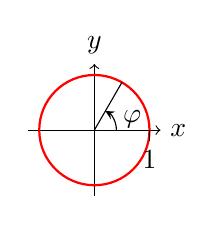
\begin{tikzpicture}[scale=0.7]
   \draw[->] (-1.2, 0) -- (1.2, 0) node[right] {$x$};
   \draw[->] (0, -1.2) -- (0, 1.2) node[above] {$y$};
  \draw[thick,red] (0,0) circle (1);
   \draw [thin] (0,0) -- (60:1);
   \draw [thin,-stealth] (0.4,0) arc (0:60:0.4) node[midway,right]{$\varphi$};
   \draw [thin] (1,0) -- (1,-0.2) node[below]{$1$};
 \end{tikzpicture}


  \item und das \alert{\enquote{Vertikaldiagramm}} (für \(\varphi=0\)); \alert{\enquote{Rückwärtskeule}} wird mitgezeichnet
    
\hspace*{1cm}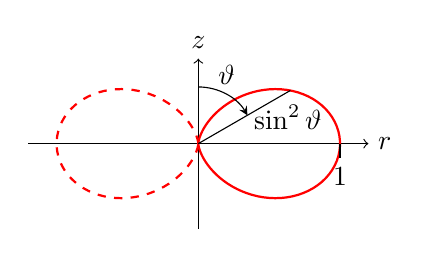
\begin{tikzpicture}[scale=1.8]
   \draw[->] (-1.2, 0) -- (1.2, 0) node[right] {$r$};
   \draw[->] (0, -0.6) -- (0, 0.6) node[above] {$z$};
  \draw[thick,red,variable=\th,domain=0:180,samples=90]
   plot ( {(sin(\th))^3} , {cos(\th)*(sin(\th))^2} );
  \draw[thick, dashed,red,variable=\th,domain=0:180,samples=90]
   plot ( {-(sin(\th))^3} , {cos(\th)*(sin(\th))^2} );
   \draw [thin] (0,0) -- (30:{(sin(60))^2}) node[midway, right]{$\sin^2\vartheta$};
   \draw [thin,-stealth] (0,0.4) arc (90:30:0.4) node[midway,above]{$\vartheta$};
   \draw [thin] (1,0) -- (1,-0.1) node[below]{$1$};
 \end{tikzpicture}
 \end{itemize}
  \end{frame}

\begin{frame}
  \frametitle{Mittlere abgestrahlte Leistung}
  \begin{itemize}[<+->]
  \item Die mittlere abgestrahlte Leistung \(\langle P_a \rangle\) ergibt sich direkt aus der mittleren Energieflussdichte integriert über die Oberfläche einer Kugel mit Radius \(r\) (\(O(K_r)\)):
    \begin{align*}
      \langle P_a \rangle &= \oiint_{O(K_r)} \textcolor{red}{\langle \poyvec[v] \rangle} \cdot \textcolor{green}{\upd\vec{A}} \\
      &= \int_0^{2\pi}\int_0^\pi \textcolor{red}{\frac{1}{2} Z \left( \frac{1}{4\pi} \frac{\omega^2}{\geschw_p^2}\frac{|\underline{I}| \ell}{\wellenzahl\ortsvektor} \right)^2 \left(\sin\vartheta\right)^2 \; \einheitsvek{r}} \cdot \textcolor{green}{\einheitsvek{r} r^2\sin\vartheta \upd\varphi\upd\vartheta}  \\
      &= \frac{1}{2} Z \left( \frac{1}{4\pi} \frac{\omega^2}{\geschw_p^2}\frac{|\underline{I}| \ell}{\wellenzahl} \right)^2 2\pi \frac{4}{3} = \frac{1}{12\pi} Z \left( \frac{\omega}{\geschw_p}|\underline{I}| \ell \right)^2 = \frac{\pi}{3} Z \left( \frac{|\underline{I}| \ell}{\lambda} \right)^2 
    \end{align*}
  \item Ein (hypothetischer) \alert{isotroper Strahler} würde pro Raumwinkel somit die Leistung \(P_{iso}= \nicefrac{\langle P_a \rangle}{4\pi r^2} \) abstrahlen.
  \item Für den Hertzschen Dipol ergibt sich so die \alert{Direktivität} (Richtwirkung)
    \begin{equation*}
      D(\vartheta,\varphi) = \frac{\poyvec_r(r,\vartheta, \varphi)}{P_{iso}} = \frac{3}{2} \sin^2\vartheta \; ; \; D_{max} = D(\vartheta=\frac{\pi}{2}) = \frac{3}{2} \hateq 1.76\; \text{dBi} \hateq 0\; \text{dBd}  
      \end{equation*}
 \end{itemize}
  \end{frame}

\begin{frame}
  \frametitle{Bemerkungen}
  \begin{itemize}[<+->]
  \item Der \alert{isotrope Strahler} ist nur eine hypothetische Idealisierung
  \item Mathematische Topologie: \enquote{Igelsatz} bzw. Satz von Poincaré-Brouwer:

    Auf einer Sphäre \(\mathbb{S}^{n}\) gibt es genau dann ein tangentiales, stetiges, nirgends verschwindendes Vektorfeld, wenn \(n\) ungerade ist.

  \item Auf der Kugel (\(n=2\)): \alert{\enquote{Jeder stetig gekämmte Igel hat mindestens einen Glatzpunkt.}}
  \item Der ideale Hertzsche Dipol kann durch extrem kurze Antennen (\(\ell < \frac{\lambda}{10}\)) tatsächlich \alert{näherungsweise} realisiert werden.
  \item Sowohl der Hertzsche Dipol als auch der isotrope Strahler werden als Bezugsgrößen in der Antennentechnik genutzt (\alert{Elementarquellen}).
  \item Das zum Hertzschen Dipol \alert{duale} System ist der \alert{Fitzgeraldsche Dipol}: infinitisimale Leiterschleife; Flächennormale in \(z\)-Richtung \(\to\) nur \(\efeld[uv]_\varphi\) und \(\magfeld[uv]_\vartheta\) im Fernfeld.
  \item Feldwellenwiderstand \(Z=\frac{|\efeld[uv]|}{|\magfeld[uv]|}\) nur im Fernfeld konstant mit \(Z=\SI{120\pi}{\ohm}\).

    Im Nahfeld des Hertzschen Dipols: \alert{Hochimpedanzfeld}

    Im Nahfeld des Fitzgeraldschen Dipols: \alert{Niederimpedanzfeld}
  \item \alert{Grenze zum Fernfeld} bei kurzen Antennen: \(\wellenzahl \ortsvektor \gg 1 \to \ortsvektor \gg  \frac{\lambda}{2\pi} = \frac{\geschw_p}{2\pi f}\):
    \begin{tabular}{c||c|c|c|c|c}
      $f$ & \SI{50}{\hertz} & \SI{1}{\kilo\hertz} & \SI{100}{\mega\hertz}& \SI{1}{\giga\hertz}\\
      \hline
      $\frac{\lichtgeschw}{2\pi f}$ & \SI{954.3}{\kilo\metre} & \SI{47.8}{\kilo\metre} &\SI{0.48}{\metre} &\SI{4.8}{\centi\metre}
    \end{tabular}
  \end{itemize}
  \ 
  \end{frame}


\begin{frame}
  \frametitle{Linearantenne}
  \begin{itemize}[<+->]
  \item Bei den Elementardipolen: infinitisimales Element \(\to\) zeitlich harmonischer aber \alert{räumlicher konstanter Strom}.
  \item \alert{Lineare Antenne}: dünner perfekt leitender Draht, der von einem \alert{ortsabhängigen} (harmonischen) Wechselstrom \(\underline{I}(\ortsvektor[vs])\) durchflossen wird.
  \item Betrachte zunächst: Stromelement im Ursprung \(\to\) Hertzscher Dipol
      \begin{columns}
    \begin{column}{.35\textwidth}
  % set the plot display orientation
%synatax: \tdplotsetdisplay{\theta_d}{\phi_d}
\tdplotsetmaincoords{60}{110}

%define polar coordinates for some vector
%TODO: look into using 3d spherical coordinate system
\pgfmathsetmacro{\rvec}{.5}
\pgfmathsetmacro{\thetavec}{30}
\pgfmathsetmacro{\phivec}{60}

%start tikz picture, and use the tdplot_main_coords style to implement the display 
%coordinate transformation provided by 3dplot
\begin{tikzpicture}[scale=5,tdplot_main_coords]

%set up some coordinates 
%-----------------------
\coordinate (O) at (0,0,0);

%determine a coordinate (P) using (r,\theta,\phi) coordinates.  This command
%also determines (Pxy), (Pxz), and (Pyz): the xy-, xz-, and yz-projections
%of the point (P).
%syntax: \tdplotsetcoord{Coordinate name without parentheses}{r}{\theta}{\phi}
\tdplotsetcoord{P}{\rvec}{\thetavec}{\phivec}

%draw figure contents
%--------------------

%draw the main coordinate system axes
\draw[thick,->] (0,0,0) -- (.5,0,0) node[anchor=north east]{$x$};
\draw[thick,->] (0,0,0) -- (0,.5,0) node[anchor=north west]{$y$};
\draw[thick,->] (0,0,0) -- (0,0,.5) node[anchor=south]{$z$};

%draw a vector from origin to point (P) 
\draw[-stealth,color=red,thick] (O) -- (P) node[midway, below]{$\ortsvektor[v]$};
\draw[-stealth,color=green,thick] (P) -- +(0,0,0.2) node[above]{$\upd\magvekpot[uv]=\upd\magvekpot[u]_z\einheitsvek{z}$};

%draw projection on xy plane, and a connecting line
\draw[dashed, color=red] (O) -- (Pxy);
\draw[dashed, color=red] (P) -- (Pxy);

%draw the angle \phi, and label it
%syntax: \tdplotdrawarc[coordinate frame, draw options]{center point}{r}{angle}{label options}{label}
\tdplotdrawarc{(O)}{0.2}{0}{\phivec}{anchor=north}{$\varphi$}


%set the rotated coordinate system so the x'-y' plane lies within the
%"theta plane" of the main coordinate system
%syntax: \tdplotsetthetaplanecoords{\phi}
\tdplotsetthetaplanecoords{\phivec}

%draw theta arc and label, using rotated coordinate system
\tdplotdrawarc[tdplot_rotated_coords]{(0,0,0)}{0.3}{0}{\thetavec}{anchor=south west}{$\vartheta$}

%draw some dashed arcs, demonstrating direct arc drawing
%\draw[dashed,tdplot_rotated_coords] (\rvec,0,0) arc (0:90:\rvec);
%\draw[dashed] (\rvec,0,0) arc (0:90:\rvec);

%set the rotated coordinate definition within display using a translation
%coordinate and Euler angles in the "z(\alpha)y(\beta)z(\gamma)" euler rotation convention
%syntax: \tdplotsetrotatedcoords{\alpha}{\beta}{\gamma}
\tdplotsetrotatedcoords{\phivec}{\thetavec}{0}

%translate the rotated coordinate system
%syntax: \tdplotsetrotatedcoordsorigin{point}
\tdplotsetrotatedcoordsorigin{(P)}

%use the tdplot_rotated_coords style to work in the rotated, translated coordinate frame
%\draw[thin,tdplot_rotated_coords,->] (0,0,0) -- (.1,0,0) node[anchor=north west]{$\vu{\vartheta}$};
%\draw[thin,tdplot_rotated_coords,->] (0,0,0) -- (0,.1,0) node[anchor=west]{$\vu{\varphi}$};
%\draw[thin,tdplot_rotated_coords,->] (0,0,0) -- (0,0,.1) node[anchor=south]{$\vu{r}$};

\node (a) [cylinder, shape border rotate=90, draw, minimum height=5mm, minimum width=2mm,yshift=-1mm] {};
\draw [<->] ([xshift=-2pt]a.before bottom) -- ([xshift=-2pt]a.after top) node [midway, left] {$\upd z^\prime$};

\end{tikzpicture}
\end{column}
\begin{column}{.65\textwidth}
  \begin{itemize}[<+->]
  \item Beitrag zum Vektorpotential am Punkt \(P\):
    \begin{equation*}
      \upd\magvekpot[uv](\ortsvektor[v]) = \frac{\mu}{4\pi} \underline{I} \upd z^\prime \frac{\euler^{-\komplex\wellenzahl\ortsvektor}}{\ortsvektor} \einheitsvek{z}
    \end{equation*}
  \item Für das Magnetfeld
    \begin{align*}
      \upd\magfeld[uv](\ortsvektor[v]) &= \frac{1}{\mu} \rotation \upd\magvekpot[uv](\ortsvektor[v])\\
      &= \frac{1}{4\pi} \underline{I} \upd z^\prime \rotation\left(\frac{\euler^{-\komplex\wellenzahl\ortsvektor}}{\ortsvektor} \einheitsvek{z}\right)
      \end{align*}
      \end{itemize}
\end{column}
\end{columns}

  \end{itemize}
  \end{frame}

\begin{frame}
  \frametitle{Magnetfeld}
  \begin{itemize}[<+->]
  \item Wir formen weiter um:
        \begin{align*}
          \upd\magfeld[uv](\ortsvektor[v])  &= \frac{1}{4\pi}\underline{I} \upd z^\prime \rotation_{\textcolor{green}{\ortsvektor}}\left(\frac{\euler^{-\komplex\wellenzahl\ortsvektor}}{\ortsvektor} \einheitsvek{z}\right) \\
                                            &= \frac{1}{4\pi} \underline{I}\upd z^\prime \bigg[ \frac{\euler^{-\komplex\wellenzahl\ortsvektor}}{\ortsvektor} \underbrace{\rotation \einheitsvek{z}}_{=\vec{0}} - \einheitsvek{z} \times \textcolor{red}{\gradient\left( \frac{\euler^{-\komplex\wellenzahl\ortsvektor}}{\ortsvektor} \right)}\bigg] \\
          &= \frac{1}{4\pi} \underline{I}\upd z^\prime \bigg[- \einheitsvek{z} \times \textcolor{red}{\left( -\frac{\ortsvektor[v]}{\ortsvektor} \left(\frac{1}{\ortsvektor} +\komplex\wellenzahl \right)   \right) \frac{\euler^{-\komplex\wellenzahl\ortsvektor}}{\ortsvektor}} \bigg]\\
          &= \frac{1}{4\pi} \underline{I}\upd z^\prime \left( \einheitsvek{z} \times \frac{\ortsvektor[v]}{\ortsvektor} \right) \left(\frac{1}{\ortsvektor} +\komplex\wellenzahl \right) \frac{\euler^{-\komplex\wellenzahl\ortsvektor}}{\ortsvektor} 
        \end{align*}
      \item Stromelement beliebiger Länge: \(\underline{I}\to \underline{I}(\ortsvektor[vs])\), \(\upd z^\prime \einheitsvek{z} \to \upd\ortsvektor[vs]\), \(\ortsvektor[v] \to \ortsvektor[v] - \ortsvektor[vs]\):
        \begin{equation*}
          \boxed{\upd\magfeld[uv](\ortsvektor[v]) = \frac{1}{4\pi} \underline{I}(\ortsvektor[vs]) \left( \upd\ortsvektor[vs] \times \frac{\ortsvektor[v]-\ortsvektor[vs]}{|\ortsvektor[v]-\ortsvektor[vs]|} \right) \left(\frac{1}{|\ortsvektor[v]-\ortsvektor[vs]|} +\komplex\wellenzahl \right) \frac{\euler^{-\komplex\wellenzahl |\ortsvektor[v]-\ortsvektor[vs]|}}{|\ortsvektor[v]-\ortsvektor[vs]|}}
          \end{equation*}
  \end{itemize}
  \end{frame}


\begin{frame}
  \frametitle{Fernfeld}
        \begin{equation*}
          \upd\magfeld[uv](\ortsvektor[v]) = \frac{1}{4\pi} \underline{I}(\ortsvektor[vs]) \left( \upd\ortsvektor[vs] \times \frac{\ortsvektor[v]-\ortsvektor[vs]}{|\ortsvektor[v]-\ortsvektor[vs]|} \right) \left(\frac{1}{|\ortsvektor[v]-\ortsvektor[vs]|} +\komplex\wellenzahl \right) \frac{\euler^{-\komplex\wellenzahl |\ortsvektor[v]-\ortsvektor[vs]|}}{|\ortsvektor[v]-\ortsvektor[vs]|}
          \end{equation*}
  \begin{itemize}[<+->]
  \item Fernfeld: Folgende Näherungen sind möglich (vgl. auch \alert{Elektromagnetische Wellen XI - Erzeugung} - Strahlungszonen)
    \begin{align*}
      \wellenzahl |\ortsvektor[v]-\ortsvektor[vs]| \gg 1 &\Rightarrow \wellenzahl \gg \frac{1}{|\ortsvektor[v]-\ortsvektor[vs]|}\\
      \frac{\ortsvektor[v]-\ortsvektor[vs]}{|\ortsvektor[v]-\ortsvektor[vs]|} &\simeq \frac{\ortsvektor[v]}{\ortsvektor}\\
      \frac{\euler^{-\komplex\wellenzahl |\ortsvektor[v]-\ortsvektor[vs]|}}{|\ortsvektor[v]-\ortsvektor[vs]|} &\simeq \frac{\euler^{-\komplex\wellenzahl \ortsvektor}}{\ortsvektor} \euler^{\komplex\wellenzahl \frac{\ortsvektor[v]\cdot \ortsvektor[vs]}{\ortsvektor}}
    \end{align*}
  \item damit gilt im \alert{Fernfeld}:
            \begin{equation*}
          \boxed{\upd\magfeld[uv](\ortsvektor[v]) = \frac{\komplex\wellenzahl}{4\pi} \underline{I}(\ortsvektor[vs]) \left( \upd\ortsvektor[vs] \times \frac{\ortsvektor[v]}{\ortsvektor} \right) \frac{\euler^{-\komplex\wellenzahl \ortsvektor}}{\ortsvektor} \euler^{\komplex\wellenzahl \frac{\ortsvektor[v]\cdot \ortsvektor[vs]}{\ortsvektor}}}
          \end{equation*}

  \end{itemize}
  \end{frame}

\begin{frame}
  \frametitle{Fernfeld (\dots)}
            \begin{equation*}
          \upd\magfeld[uv](\ortsvektor[v]) = \frac{\komplex\wellenzahl}{4\pi} \underline{I}(\ortsvektor[vs]) \left( \upd\ortsvektor[vs] \times \frac{\ortsvektor[v]}{\ortsvektor} \right) \frac{\euler^{-\komplex\wellenzahl \ortsvektor}}{\ortsvektor} \euler^{\komplex\wellenzahl \frac{\ortsvektor[v]\cdot \ortsvektor[vs]}{\ortsvektor}}
          \end{equation*}
  \begin{itemize}[<+->]
  \item Dünner Draht mit Kontur \(C\):
    \bigskip
    
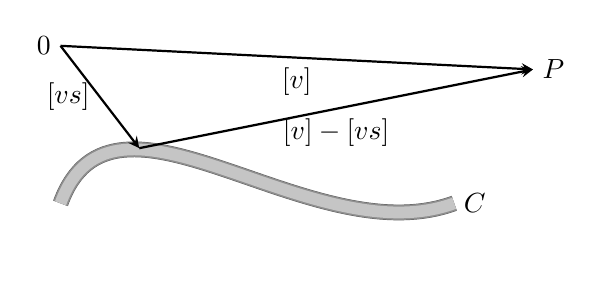
\begin{tikzpicture}
  \Tube{2mm}{3}{gray!25}{black!75}{(0,2) to[out=70,in=200] (5,2)}
  \draw (5,2) node[right]{$C$};
  \draw (0,4) node[left]{$0$}; 
  \draw (6,3.7) node[right]{$P$}; 
    \draw[-stealth,thick] (0,4) -- (1,2.7) node[midway,left]{$\ortsvektor[vs]$}; 
    \draw[-stealth,thick] (0,4) -- (6,3.7) node[midway,below]{$\ortsvektor[v]$}; 
    \draw[-stealth,thick] (1,2.7) -- (6,3.7) node[midway,below]{$\ortsvektor[v]-\ortsvektor[vs]$}; 
\end{tikzpicture}
\item Damit ist das Magnetfeld im Fernfeld prinzipiell berechenbar aus:
            \begin{equation*}
          \boxed{\magfeld[uv](\ortsvektor[v]) = \frac{\komplex\wellenzahl}{4\pi} \frac{\euler^{-\komplex\wellenzahl \ortsvektor}}{\ortsvektor} \int_{C}\underline{I}(\ortsvektor[vs]) \euler^{\komplex\wellenzahl \frac{\ortsvektor[v]\cdot \ortsvektor[vs]}{\ortsvektor}} \left( \upd\ortsvektor[vs] \times \frac{\ortsvektor[v]}{\ortsvektor} \right)} 
          \end{equation*}
  \end{itemize}
  \end{frame}

  \begin{frame}
  \frametitle{Abstrahldiagramme typischer Dipol-Antennen}
\centerline{\includegraphics[height=.8\textheight]{Lineare_Dipole}}
  \end{frame}

    \begin{frame}
  \frametitle{Typische Bauformen von Linearantennen}
\centerline{\includegraphics[width=\textwidth]{Antennen-Bilder}}
  \end{frame}

\input{finalframe.inc}
   
\end{document}